\documentclass{beamer}
\usepackage{hyperref}
\usepackage[T1]{fontenc}

% other packages
\usepackage{latexsym,amsmath,xcolor,multicol,booktabs,calligra}
\usepackage{graphicx,pstricks,listings,stackengine}

% dummy text; remove it when working on this template
\usepackage{lipsum}


\author{Ayush Raina, Anushka Dassi, Arnav Bhatt}
\title{Variational Autoencoders}
\subtitle{A Deep Generative Model}
\institute{
    Indian Institute of Science \\
}
\date{\today}
\usepackage{Ritsumeikan} 


% defs
\def\cmd#1{\texttt{\color{red}\footnotesize $\backslash$#1}}
\def\env#1{\texttt{\color{blue}\footnotesize #1}}
\definecolor{deepblue}{rgb}{0,0,0.5}
\definecolor{deepred}{RGB}{153,0,0}
\definecolor{deepgreen}{rgb}{0,0.5,0}
\definecolor{halfgray}{gray}{0.55}

\lstset{
    basicstyle=\ttfamily\small,
    keywordstyle=\bfseries\color{deepblue},
    emphstyle=\ttfamily\color{deepred},    % Custom highlighting style
    stringstyle=\color{deepgreen},
    numbers=left,
    numberstyle=\small\color{halfgray},
    rulesepcolor=\color{red!20!green!20!blue!20},
    frame=shadowbox,
}

\begin{document}

\begin{frame}
    \titlepage
\end{frame}
    
\section*{Autoencoders}
\begin{frame}{What are Autoencoders ?}
1. Autoencoders are neural networks that aim to learn the compact representation of the input data whose dimension is much smaller than the input data.\\
2. It consists of two parts: an $encoder(\phi)$ and a $decoder(\theta)$, where encoder and decoder are neural networks.\\

\pause

\begin{block}{Goal}
    The goal of encoder network is to learn a hidden representation of the input data, and the goal of decoder network is to reconstruct the input data from the hidden representation.
\end{block}
\end{frame}

\begin{frame}{Training Autoencoders}
    \begin{itemize}
        \item The training of autoencoders is done by minimizing the reconstruction error between the input data and the reconstructed data.
        \item The loss function used for training autoencoders is Mean Squared Error (MSE).
        \pause
        \item The loss function is given by:
        \begin{equation}
            \boxed{L(\phi, \theta) = \frac{1}{N} \sum_{i=1}^{N} ||x_i - Decoder_{\theta}(Encoder_{\phi}(x_i))||^2}
        \end{equation}
        where $x_i$ is the input data, $Encoder_{\phi}(x_i)$ is the hidden representation of $x_i$ and $Decoder_{\theta}(Encoder_{\phi}(x_i))$ is the reconstructed data.
    \end{itemize}
    
\end{frame}

\begin{frame}{Reconstructions of Autoencoders}
    \begin{figure}
        \centering
        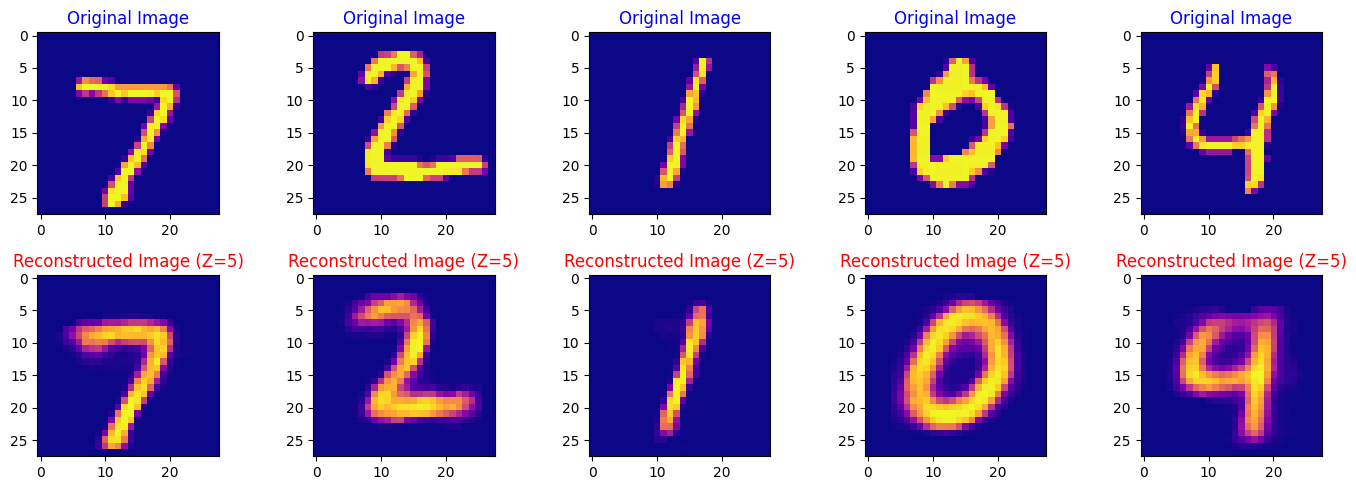
\includegraphics[width=0.5\textwidth]{../ReportNeurips/autoencoder1.png}
        \caption{Reconstruction of Autoencoders without CNN}
    \end{figure}

    \begin{figure}
        \centering
        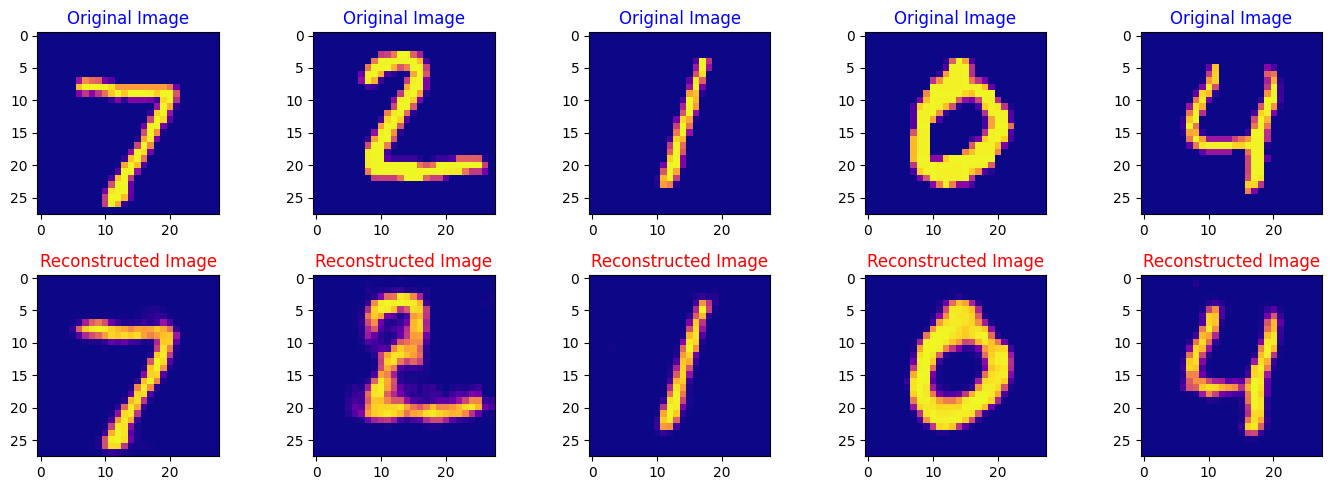
\includegraphics[width=0.5\textwidth]{../ReportNeurips/autoencoder2.png}
        \caption{Reconstruction of Autoencoders with CNN}
    \end{figure}

    In both the cases we trained for over 20 epochs.
\end{frame}

\begin{frame}{Reconstructions of Autoencoders}
    \begin{figure}
        \centering
        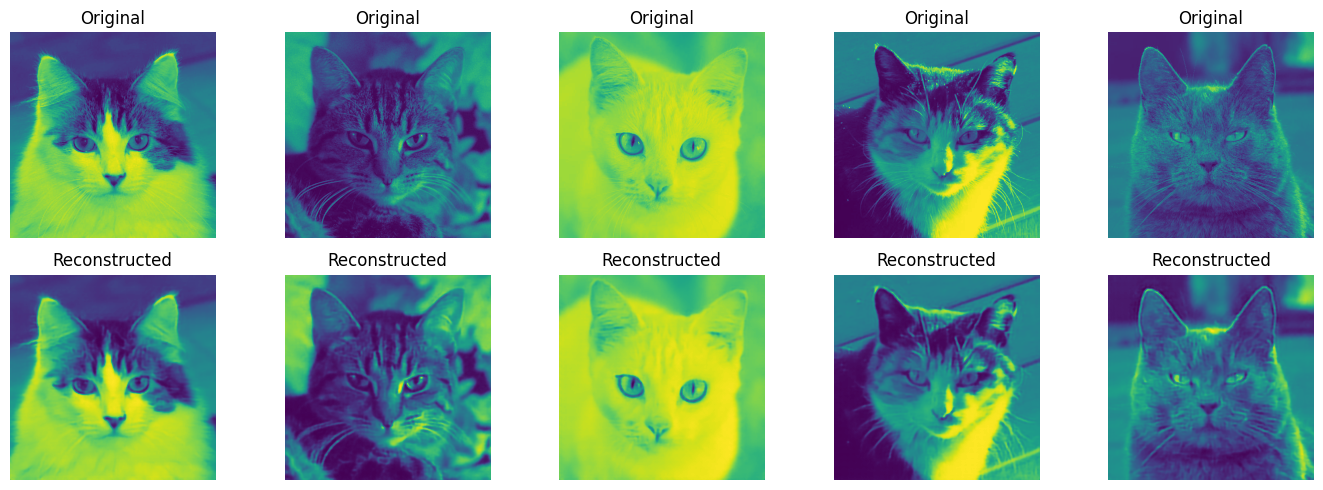
\includegraphics[width=0.8\textwidth]{../ReportNeurips/animalFaceAE1.png}
        \caption{Reconstruction of Autoencoders on Animal Face Dataset}
    \end{figure}
    This reconstruction was done on grayscale version, we also obtained similar output on colored version.
\end{frame}
\begin{frame}{Generation}
    \begin{block}{Can we generate new data with Autoencoders ?}
        After the training of autoencoders, we can generate new data by feeding random hidden representation to the decoder network. But we may simply get noise in the output.
    \end{block}
    This is because the hidden representation lies in very small subspace of the input space.
\end{frame}

\begin{frame}{Generation}
    \begin{figure}
        \centering
        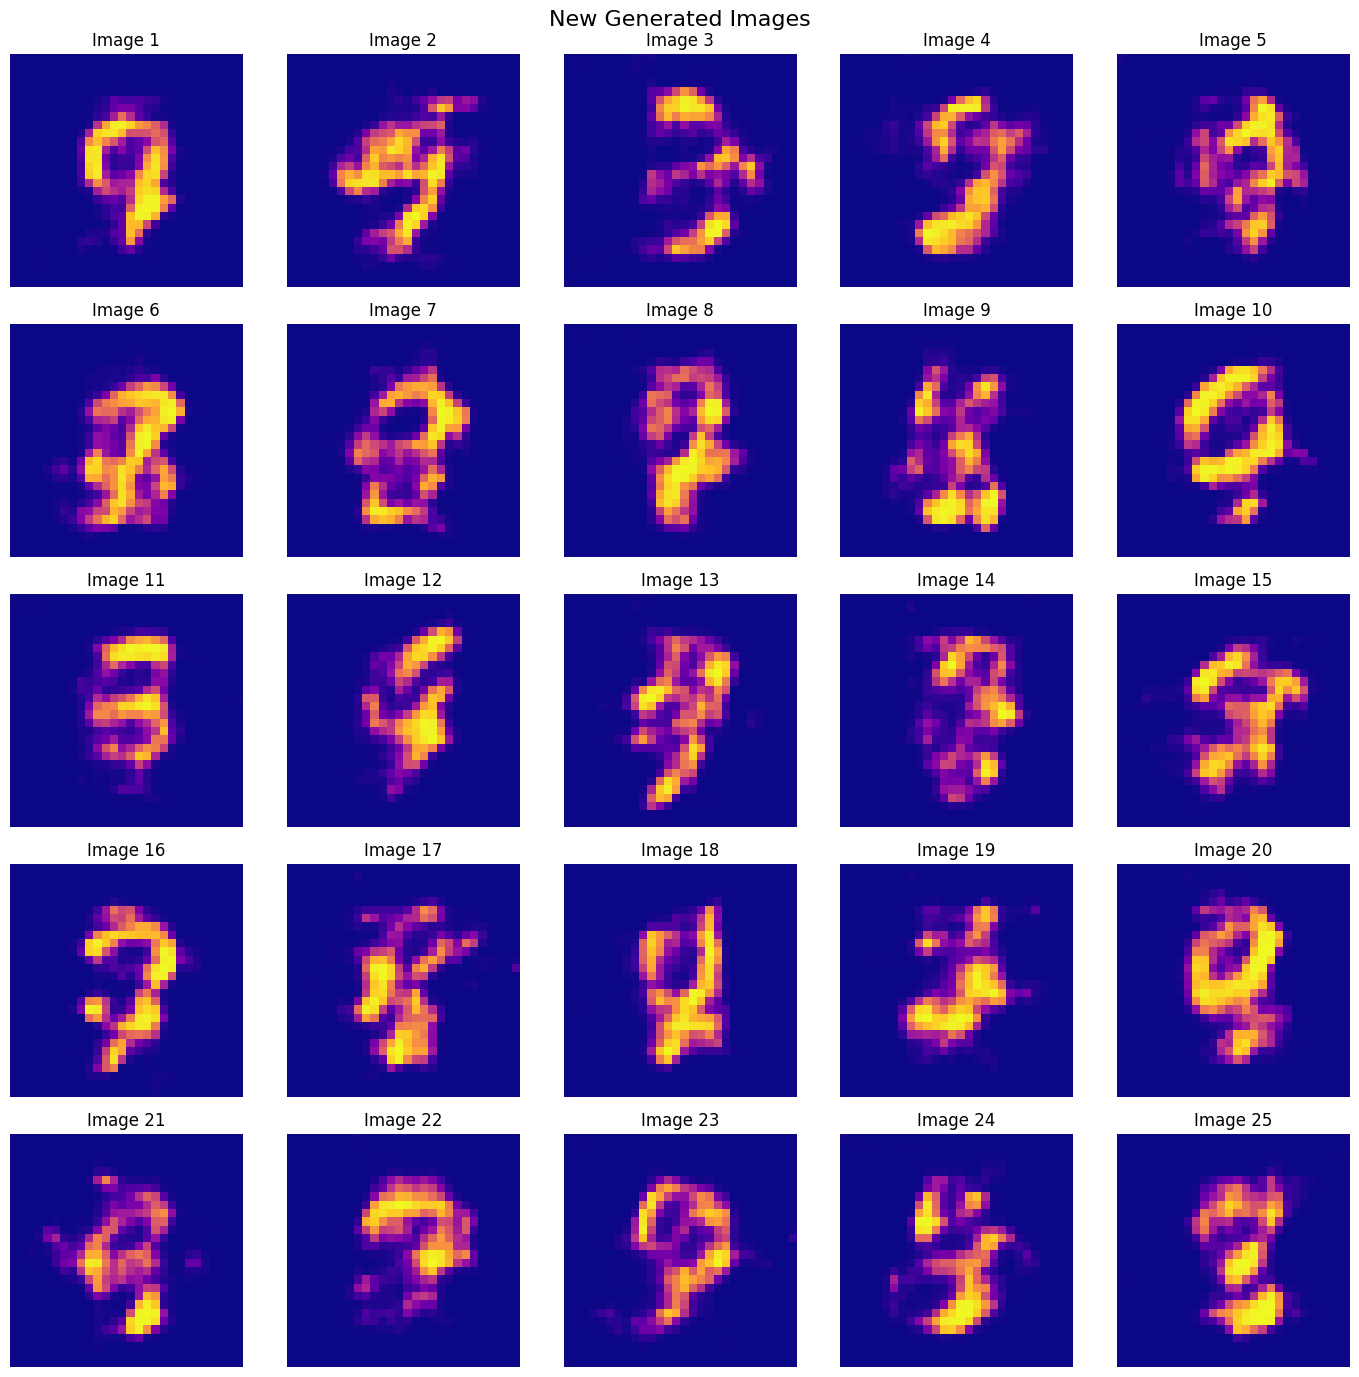
\includegraphics[width=0.3\textwidth]{../ReportNeurips/mnistGenerated2.png}
        \caption{Generation of new handwritten digits using Autoencoders}
    \end{figure}
    \pause
    This is the generation when we fed \textcolor{red}{mean} of the hidden representations generated by the encoder network. Otherwise output was simply a noise.
\end{frame}

\begin{frame}{Generation}
    \begin{block}{What should be done ?}
        If we somehow feed the highly likely hidden representation $z$, then we can expect meaningful output.
    \end{block}
\end{frame}

\begin{frame}{Generation}
    \begin{block}{What is highly likely hidden representation ?}
        In fact we want to sample from $P(z^{(i)}|x^{(i)})$ where $z^{(i)}$ is the hidden representation of $x^{(i)}$.
    \end{block}
    Here both encoder and decoder networks are deterministic, which means for every input data $x^{(i)}$, the hidden representation $z^{(i)}$ is fixed and vice versa.
\end{frame}
\section*{Variational Autoencoders}

\begin{frame}{Setting up the problem}
    
\end{frame}


\section*{Experimental Results}
\begin{frame}{VAE's on MNIST Dataset}

\end{frame}
\section*{EM Algorithm}
\begin{frame}{Expectation Maximisation Algorithm}

\end{frame}

\begin{frame}{Problems with EM Algorithm}
    
\end{frame}

\begin{frame}{Solution: Variational Inference}

\end{frame}


% thank you slide
\begin{frame}{Thank You!}
    \begin{center}
        \Huge Thank You!
    \end{center}
    Here are some references:
    \begin{enumerate}
        \item ELBO Surgery: Yet Another Way to Carve Up the Variational Evidence Lower Bound, \url{https://approximateinference.org/2016/accepted/HoffmanJohnson2016.pdf}
        \item CS229 Lecture Notes for VAE, \url{https://cs229.stanford.edu/summer2019/cs229-notes8.pdf}
        \item Tutorial on Variational Autoencoders, \url{https://arxiv.org/pdf/1606.05908.pdf}
    \end{enumerate}
\end{frame}

\end{document}

